\documentclass{article}
\usepackage[T1]{fontenc}
\usepackage{lmodern}
\usepackage[polish]{babel}
\usepackage{graphicx}
\usepackage{float}
\usepackage{hyperref}
\usepackage{enumitem}
\usepackage{amsmath}
\usepackage{caption}
\usepackage{subcaption}
\usepackage{xcolor}

\usepackage[a4paper, margin=2.54cm]{geometry}

\title{Egzamin zerowy - sprawozdanie}
\author{Damian Jankowski s188597}

\begin{document}

\maketitle

\tableofcontents

\section{Zadanie 1 - Układ rozmyty}

\subsection{Wstęp}

Układy rozmyte, znane również jako logika rozmyta, 
to gałąź teorii sterowania i sztucznej inteligencji, 
która umożliwia modelowanie i sterowanie systemami, 
charakteryzującymi się nieprecyzyjnymi lub niejednoznacznymi danymi. 
W odróżnieniu od tradycyjnych podejść logicznych, 
które operują na wartościach prawda/fałsz, 
logika rozmyta umożliwia wyrażanie i manipulację stopniami 
przynależności, które mogą przyjmować wartości z przedziału $[0, 1]$.
Pozwala to na wyrażanie niepewności i niejednoznaczności w sposób 
bardziej naturalny.

\subsubsection{Funkcje przynależności}

Funkcje przynależności służą do opisu stopnia przynależności obiektów 
do zbiorów rozmytych. Przykładowo, można zdefiniować funkcję 
przynależności \textit{wysoki} dla wzrostu człowieka, która będzie miała 
wartość bliską 1 dla osób bardzo wysokich i wartość bliską 0 dla 
osób niskich. Wartości pośrednie będą odpowiadały osobom o
średnim wzroście. Wyróżnia się kilka rodzajów funkcji
przynależności, m.in. trójkątną, trapezoidalną, gaussowską,
sigmoidalną, typu s, z czy $\pi$.

\subsubsection{Operacje na zbiorach rozmytych}

Operacje na zbiorach rozmytych obejmują operacje algebraiczne, 
takie jak unia, przecięcie i dopełnienie zbiorów rozmytych. 
Te operacje umożliwiają manipulację stopniami przynależności 
i pozwalają na wykonywanie operacji logicznych na zmiennych rozmytych.

Najważniejszymi z nich są operacje unii i przecięcia, które
pozwalają na wyznaczenie stopnia przynależności do zbioru
wynikowego na podstawie stopni przynależności do zbiorów
pierwotnych. W przypadku operacji unii, stopień przynależności
do zbioru wynikowego jest równy maksimum stopni przynależności
do zbiorów pierwotnych, natomiast w przypadku operacji przecięcia
jest to minimum.

\begin{equation}
    \mu_{A \cup B}(x) = \max(\mu_A(x), \mu_B(x))
\end{equation}

\begin{equation}
    \mu_{A \cap B}(x) = \min(\mu_A(x), \mu_B(x))
\end{equation}

\subsubsection{Etapy użycia układu rozmytego} \label{sec:etapy}

\begin{enumerate}
    \item Rozmywanie - przekształcenie danych wejściowych na zmienne rozmyte
    \item Operacje rozmyte - wykonanie operacji logicznych na zmiennych rozmytych
    \item Implikacje - wyznaczenie stopni przynależności dla każdej reguły wybraną
    metodą wnioskowania, np. metodą Mamdaniego, która polega na wyznaczeniu
    minimum stopni przynależności do zbiorów rozmytych dla każdej reguły
    \item Kompozycja - połączenie wynikowych zbiorów rozmytych w celu uzyskania 
    jednego zbioru rozmytego. Wyróżnia się dwie metody kompozycji:
    \begin{enumerate}
        \item Metoda MAX - wybór maksymalnej wartości z funkcji przynależności otrzymanych dla
        wszystkich reguł
        \item Metoda SUM - wynikowa funkcja przynależności jest sumą funkcji przynależności
        otrzymanych dla wszystkich reguł
    \end{enumerate}
    \item Precyzowanie - obliczenie konkretnej wartości na podstawie otrzymanej funkcji przynależności.
    Do tego celu wyznacza się środek ciężkości funkcji przynależności zdefiniowany jako:
    \begin{equation}
        s_c = \frac{\int_{a}^{b} x s(x) dx}{\int_{a}^{b} s(x) dx}
    \end{equation}
\end{enumerate}

\subsection{Wybrany układ rozmyty}

Do realizacji zadania zdecydowałem się na zaprojektowanie
układu sterowania klimatyzacji. Układ sterowania klimatyzacji
wymaga dwóch wejść: temperatury i wilgotności. Na podstawie
tych danych układ sterowania musi wyznaczyć moc klimatyzatora,
która będzie odpowiednia do utrzymania prawidłowych warunków
w pomieszczeniu. W tym celu należy zdefiniować:
\begin{itemize}
    \item Reguły sterowania, które będą określać moc klimatyzatora
    w zależności od temperatury i wilgotności
    \item Zbiory rozmyte dla każdego z parametrów oraz 
    ich funkcje przynależności
\end{itemize}

\subsubsection*{Reguły sterowania}

\begin{enumerate}[label=Reguła \arabic*:, leftmargin=*]
    \item Jeśli temperatura jest niska, to moc jest niska
    \item Jeśli temperatura jest wysoka i wilgotność jest niska, to moc jest średnia
    \item Jeśli temperatura jest wysoka i wilgotność jest wysoka, to moc jest wysoka
\end{enumerate}

\subsubsection*{Zbiory rozmyte oraz funkcje przynależności}

\begin{table}[H]
    \centering
    \begin{tabular}{|c|c|c|}
        \hline
        \textbf{Nazwa zbioru} & \textbf{Funkcja przynależności} & \textbf{Zakres zmiennej} \\
        \hline
        "temperatura niska" & \textit{tn} & $[10, 30 ^\circ C]$ \\
        "temperatura wysoka" & \textit{tw} & $[10, 30 ^\circ C]$ \\
        "wilgotność niska" & \textit{wn} & $[0, 100 \%]$ \\
        "wilgotność wysoka" & \textit{ww} & $[0, 100 \%]$ \\
        "moc niska" & \textit{mn} & $[0, 100 \%]$ \\
        "moc średnia" & \textit{ms} & $[0, 100 \%]$ \\
        "moc wysoka" & \textit{mw} & $[0, 100 \%]$ \\
        \hline
    \end{tabular}
\end{table}

\begin{equation*}
    tn(x) = \begin{cases}
        1 & \text{dla } x \leq 10 \\
        \frac{30 - x}{20} & \text{dla } 10 < x < 30 \\
        0 & \text{dla } x \geq 30
    \end{cases}, \quad
    tw(x) = \begin{cases}
        0 & \text{dla } x \leq 10 \\
        \frac{x - 10}{20} & \text{dla } 10 < x < 30 \\
        1 & \text{dla } x \geq 30
    \end{cases}
\end{equation*}

\begin{equation*}
    wn(x) = \begin{cases}
        1 & \text{dla } x \leq 40 \\
        \frac{100 - x}{60} & \text{dla } 40 < x < 100 \\
        0 & \text{dla } x \geq 100
    \end{cases}, \quad
    ww(x) = \begin{cases}
        0 & \text{dla } x \leq 60 \\
        \frac{x - 40}{60} & \text{dla } 40 < x < 100 \\
        1 & \text{dla } x \geq 100
    \end{cases}
\end{equation*}

\begin{equation*}
    mn(x) = \begin{cases}
        1 & \text{dla } x \leq 30 \\
        \frac{70 - x}{40} & \text{dla } 30 < x < 70 \\
        0 & \text{dla } x \geq 70
    \end{cases}, \quad
    ms(x) = \begin{cases}
        0 & \text{dla } x \leq 20 \\
        \frac{x - 20}{30} & \text{dla } 20 < x \leq 50 \\
        \frac{80 - x}{30} & \text{dla } 50 < x < 80 \\
        0 & \text{dla } x \geq 80
    \end{cases}
\end{equation*}

\begin{equation*}
    mw(x) = \begin{cases}
        0 & \text{dla } x \leq 30 \\
        \frac{x - 30}{40} & \text{dla } 50 < x < 70 \\
        1 & \text{dla } x \geq 70
    \end{cases}
\end{equation*}

\begin{figure}[H]
    \centering
    \begin{subfigure}{0.45\textwidth}
        \centering
        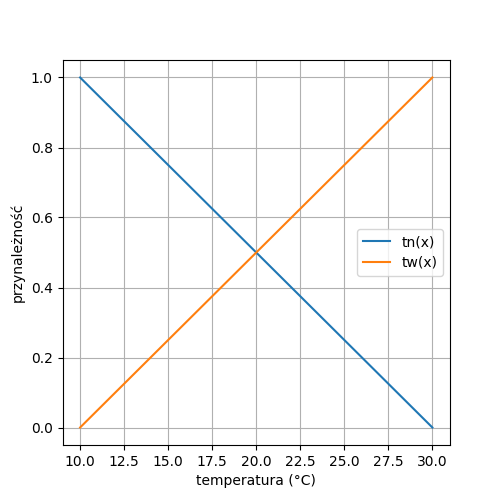
\includegraphics[width=\linewidth]{Zad1/tn_tw.png}
        \caption{Funkcje przynależności dla temperatury}
    \end{subfigure}
    \hfill
    \begin{subfigure}{0.45\textwidth}
        \centering
        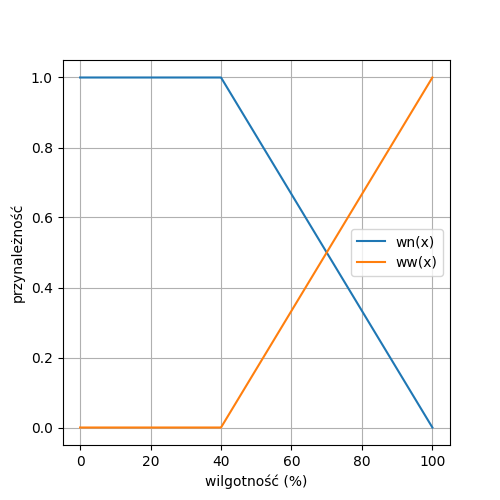
\includegraphics[width=\linewidth]{Zad1/wn_ww.png}
        \caption{Funkcje przynależności dla wilgotności}
    \end{subfigure}
    
    \vspace{1cm}
    
    \begin{subfigure}{0.45\textwidth}
        \centering
        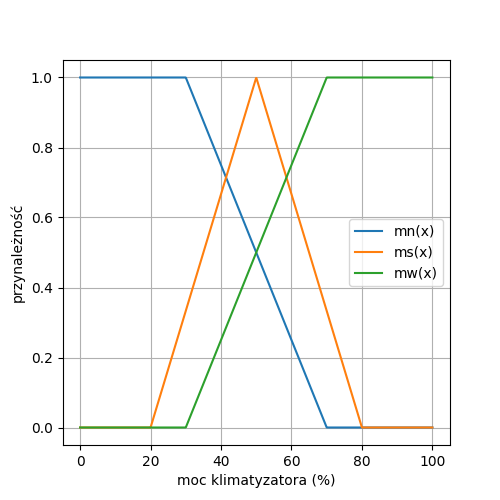
\includegraphics[width=\linewidth]{Zad1/mn_ms_mw.png}
        \caption{Funkcje przynależności dla mocy}
    \end{subfigure}
    \caption{Funkcje przynależności dla różnych zmiennych}
\end{figure}

\subsubsection{Zadanie}

Przypuśćmy, że w pomieszczeniu panują następujące warunki:
\begin{itemize}
    \item Temperatura: $T = 25 ^\circ C$
    \item Wilgotność: $W = 65 \%$
\end{itemize}
Naszym zadaniem jest określenie jaka powinna być moc klimatyzatora.

Postępujemy zgodnie z krokami opisanymi w rozdziale \ref{sec:etapy}.

\subsubsection*{Rozmywanie}

\begin{enumerate}[label=Reguła \arabic*:, leftmargin=*]
    \item $tn(25) = \frac{30 - 25}{20} = 0.25$
    \item $tw(25) = \frac{25 - 10}{20} = 0.75$ oraz $wn(65) = \frac{100 - 65}{60} = 0.58$
    \item $tw(25) = 0.75$ oraz $ww(65) = \frac{65 - 40}{60} = 0.42$
\end{enumerate}

\subsubsection*{Operacje rozmyte}

\begin{enumerate}[label=Reguła \arabic*:, leftmargin=*]
    \item $tn(25) = \frac{30 - 25}{20} = 0.25$
    \item $min(tw(25), wn(65)) = min(0.75, 0.58) = 0.58$
    \item $min(tw(25), ww(65)) = min(0.75, 0.42) = 0.42$
\end{enumerate}

\subsubsection*{Implikacje}
Ograniczamy funkcje przynależności do wartości obliczonych 
w poprzednim kroku.
\begin{enumerate}[label=Reguła \arabic*:, leftmargin=*]
    \item $mn(x) = 0.25 => \frac{70 - x}{40} = 0.25 => x = 60$
    \item $ms(x) = 0.58 => \frac{x - 20}{30} = 0.58 => x_1 = 37.4$\\
          $ms(x) = 0.58 => \frac{80 - x}{30} = 0.58 => x_2 = 62.6$
    \item $mw(x) = 0.42 => \frac{x - 30}{40} = 0.42 => x = 46.8$
\end{enumerate}

\begin{enumerate}[label=Reguła \arabic*:, leftmargin=*]
    \item $s_1(x) = \begin{cases}
        0.25 & \text{dla } x \leq 60 \\
        \frac{70 - x}{40} & \text{dla } 60 < x < 70 \\
        0 & \text{dla } x \geq 70
    \end{cases}$
    \item $s_2(x) = \begin{cases}
        0 & \text{dla } x \leq 20 \\
        \frac{x - 20}{30} & \text{dla } 20 < x \leq 37.4 \\
        0.58 & \text{dla } 37.4 < x \leq 62.6 \\
        \frac{80 - x}{30} & \text{dla } 62.6 < x < 80 \\
        0 & \text{dla } x \geq 80
    \end{cases}$
    \item $s_3(x) = \begin{cases}
        0 & \text{dla } x \leq 30 \\
        \frac{x - 30}{40} & \text{dla } 30 < x < 46.8 \\
        0.42 & \text{dla } x \geq 46.8
    \end{cases}$
\end{enumerate}

\begin{figure}[H]
    \centering
    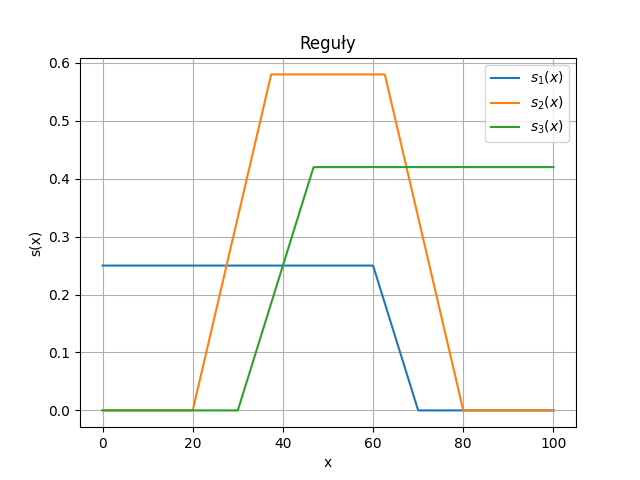
\includegraphics[width=0.8\linewidth]{Zad1/rules.png}
    \caption{Implikacje dla różnych reguł}
\end{figure}

\subsubsection*{Kompozycja}

Korzystając z metody MAX, otrzymujemy funkcję przynależności
wyniku $s(x)$:

\begin{equation}
    s(x) = \begin{cases}
        0.25 & \text{dla } x \leq 27.5 \\
        \frac{x - 20}{30} & \text{dla } 27.5 < x \leq 37.4 \\
        0.58 & \text{dla } 37.4 < x \leq 62.6 \\
        \frac{80 - x}{30} & \text{dla } 62.6 < x \leq 67.4 \\
        0.42 & \text{dla } x > 67.4 \\
    \end{cases}
\end{equation}

\begin{figure}[H]
    \centering
    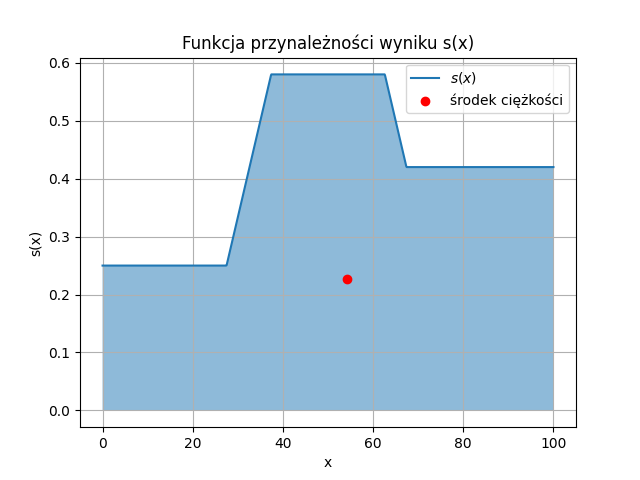
\includegraphics[width=0.8\linewidth]{Zad1/composition.png}
    \caption{Funkcja przynależności wyniku $s(x)$}
\end{figure}

\subsubsection*{Precyzowanie}

Wyznaczamy środek ciężkości $s_c$ funkcji przynależności $s(x)$:

\begin{equation}
    s_c = \frac{\int_{a}^{b} x s(x) dx}{\int_{a}^{b} s(x) dx} = 54.28786195282766
\end{equation}
Moc klimatyzatora powinna wynosić $54.23 \%$.

\subsection{Wnioski}

Model układu rozmytego w większości przypadków daje wyniki zadowalające.
Natomiast w celu uzyskania dokładniejszych wyników należałoby zwiększyć liczbę reguł,
oraz udoskonalić funkcje przynależności. Problemem może też być obliczenie środka
ciężkości funkcji przynależności wyniku, ponieważ w przypadku, gdy funkcja ma
bardzo nieregularny kształt, może być ono trudne do wyznaczenia.


\section{Zadanie 2 - Redukcja wymiarów}

Do przeprowadzenia redukcji wymiarów skorzystałem z metody PCA \textit{(Principal Component Analysis)}.
Metoda ta polega na wyznaczeniu kierunków, w których występuje największa wariancja danych.
Wyznaczone kierunki nazywamy wektorami własnymi lub głównymi składowymi. 
W celu wyznaczenia głównych składowych
wykorzystujemy macierz kowariancji. Wyznaczone główne składowe są ortogonalne do siebie.
W celu wyznaczenia nowych współrzędnych danych, należy pomnożyć macierz danych przez
macierz głównych składowych.

\subsection{Dane wejściowe}

\begin{equation}
    X = 
    \begin{bmatrix}
        \textcolor{red}{1} & \textcolor{red}{8} & \textcolor{red}{8} \\
        \textcolor{green}{5} & \textcolor{green}{9} & \textcolor{green}{7} \\
        \textcolor{blue}{3} & \textcolor{blue}{6} & \textcolor{blue}{9} \\
    \end{bmatrix}
\end{equation}

Dane wejściowe to macierz $X$ o wymiarach $3 \times 3$. Celem redukcji wymiarów
jest wyznaczenie nowej macierzy $X_{new}$ o wymiarach $3 \times 2$, nie tracąc
przy tym istotnych informacji o danych.

\subsection{Kroki algorytmu}
\subsubsection*{Standaryzacja danych}

W celu uniknięcia błędów numerycznych, dane wejściowe należy
standaryzować. Standaryzacja polega na przeskalowaniu danych
tak, aby miały średnią równą $0$ oraz odchylenie standardowe
równe $1$.

\begin{equation}
    X_{std} = \frac{X - \mu}{\sigma}
\end{equation}
gdzie: $\mu = \frac{1}{n} \sum_{i=1}^{n} x_i$ (średnia) oraz $\sigma = \sqrt{\frac{1}{n} \sum_{i=1}^{n} (x_i - \mu)^2}$
(odchylenie standardowe).

Przykładowo dla pierwszej cechy obliczenia są następujące:

\begin{equation*}
    \mu = \frac{1}{3} (1 + 5 + 3) = 3
\end{equation*}

\begin{equation*}
    \sigma = \sqrt{\frac{1}{3} ((1 - 3)^2 + (5 - 3)^2 + (3 - 3)^2)} = 1.633
\end{equation*}

\begin{table}[H]
    \centering
    \begin{tabular}{|c|c|c|c|}
        \hline
        & $x_1$ & $x_2$ & $x_3$ \\
        \hline
        $\mu$ & 3 & 7.67 & 8 \\
        \hline
        $\sigma$ & 1.633 & 1.247 & 0.816 \\
        \hline
    \end{tabular}
    \caption{Średnia oraz odchylenie standardowe danych wejściowych dla każdej cechy}
\end{table}

\begin{equation}
    X_{std} = 
    \begin{bmatrix}
        -1.2247 & 0.2672 & 0 \\
        1.2247 & 1.069 & -1.2247 \\
        0 & -1.3363 & 1.2247 \\
    \end{bmatrix}
\end{equation}

\subsubsection*{Wyznaczenie macierzy kowariancji}

Wyznaczenie macierzy kowariancji polega na obliczeniu
macierzy iloczynów skalaranych pomiędzy każdą parą cech.

\begin{equation}
    cov(X) = \begin{bmatrix}
        cov(x_1, x_1) & cov(x_1, x_2) & cov(x_1, x_3) \\
        cov(x_2, x_1) & cov(x_2, x_2) & cov(x_2, x_3) \\
        cov(x_3, x_1) & cov(x_3, x_2) & cov(x_3, x_3) \\
    \end{bmatrix}
\end{equation}

\begin{equation}
    cov(x_i, x_j) = \frac{1}{n} \sum_{k=1}^{n} (x_{ki} - \mu_i)(x_{kj} - \mu_j) \quad
    var(x_i) = \frac{1}{n} \sum_{k=1}^{n} (x_{ki} - \mu_i)^2
\end{equation}

Przyjmując założenia, że $cov(x_i, x_i) = var(x_i)$, $cov(x_i, x_j) = cov(x_j, x_i)$,
średnia każdej cechy jest równa $0$ oraz odchylenie standardowe każdej cechy jest równe $1$,
otrzymujemy przykładowe obliczenia:

\begin{equation*}
    cov(x_1, x_1) = var(x_1) = \frac{1}{3} ((-1.2247 - 0)^2 + (1.2247 - 0)^2 + (0 - 0)^2) = 1
\end{equation*}

\begin{equation*}
    cov(x_1, x_2) = \frac{1}{3} ((-1.2247 - 0)(0.2672 - 0) + (1.2247 - 0)(1.069 - 0) + (0 - 0)(-1.3363 - 0)) = 0.3273
\end{equation*}

\begin{equation}
    cov(X) = 
    \begin{bmatrix}
        1 & 0.3273 & -0.5 \\
        0.3273 & 1 & -0.9819 \\
        -0.5 & -0.9819 & 1 \\
    \end{bmatrix}
\end{equation}

\subsubsection*{Wyznaczenie wartości własnych i wektorów własnych macierzy kowariancji}

Wyznaczenie wartości własnych macierzy kowariancji
polega na rozwiązaniu równania $det(cov(X) - \lambda I) = 0$.

\begin{equation}
    det(cov(X) - \lambda I) = 
    \begin{vmatrix}
        1 - \lambda & 0.3273 & -0.5 \\
        0.3273 & 1 - \lambda & -0.9819 \\
        -0.5 & -0.9819 & 1 - \lambda \\
    \end{vmatrix} = 0
\end{equation}

\begin{equation*}
    0.00012297 - 1.6787471\lambda+3\lambda^2-\lambda^3 = 0
\end{equation*}

\begin{equation*}
    \lambda_1 = 2.2559 \quad \lambda_2 = 0.74407 \quad \lambda_3 \approx 0
\end{equation*}

Następnie należy wyznaczyć wektory własne dla każdej wartości własnej,
korzystając z równania $(cov(X) - \lambda_i I) \cdot v_i = 0$
oraz metody Cramera, podstawiając
odpowiednie wartości własne wyznaczone wcześniej.

Przykładowo dla $\lambda_1 = 2.2559$:

\begin{equation*}
    (cov(X) - \lambda_1 I) \cdot v_1 = 
    \begin{bmatrix}
        -1.2559 & 0.3273 & -0.5 \\
        0.3273 & -1.2559 & -0.9819 \\
        -0.5 & -0.9819 & -1.2559 \\
    \end{bmatrix} \cdot v_1 = 0
\end{equation*}

\begin{equation*}
    v_1 = 
    \begin{bmatrix}
        0.42397 \\
        0.62384 \\
        -0.65655 \\
    \end{bmatrix}
\end{equation*}

Dla pozostałych wartości własnych otrzymujemy następujące wektory własne:

\begin{equation*}
    v_2 = 
    \begin{bmatrix}
        0.89385 \\
        -0.40498 \\
        0.19240 \\
    \end{bmatrix}
    \quad
    v_3 = 
    \begin{bmatrix}
        0.14586 \\
        0.66843 \\
        0.72932 \\
    \end{bmatrix}
\end{equation*}

Potem należy wybrać te wektory własne, których odpowiadające im wartości własne
są największe. W tym przypadku są to $\lambda_1 = 2.2559$ oraz $\lambda_2 = 0.74407$.

\begin{equation*}
    V = 
    \begin{bmatrix}
        0.42397 & 0.89385 \\
        0.62384 & -0.40498 \\
        -0.65655 & 0.19240 \\
    \end{bmatrix}
\end{equation*}

\subsubsection*{Wyznaczenie nowych współrzędnych}

Wyznaczenie nowych, zredukowanych współrzędnych polega na pomnożeniu macierzy
znormalizowanych danych przez macierz wektorów własnych.

\begin{equation}
    X_{new} = X \cdot V
\end{equation}

\begin{equation*}
    X_{new} = 
    \begin{bmatrix}
        -1.2247 & 0.2672 & 0 \\
        1.2247 & 1.069 & -1.2247 \\
        0 & -1.3363 & 1.2247 \\
    \end{bmatrix}
    \cdot
    \begin{bmatrix}
        0.42397 & 0.89385 \\
        0.62384 & -0.40498 \\
        -0.65655 & 0.19240  \\
    \end{bmatrix}
    =
    \begin{bmatrix}
        -0.35252866 & -1.20297636 \\
        1.99028916 & 0.4261528 \\
        -1.6377605 & 0.77682356 \\
    \end{bmatrix}
\end{equation*}

\begin{figure}[H]
    \centering
    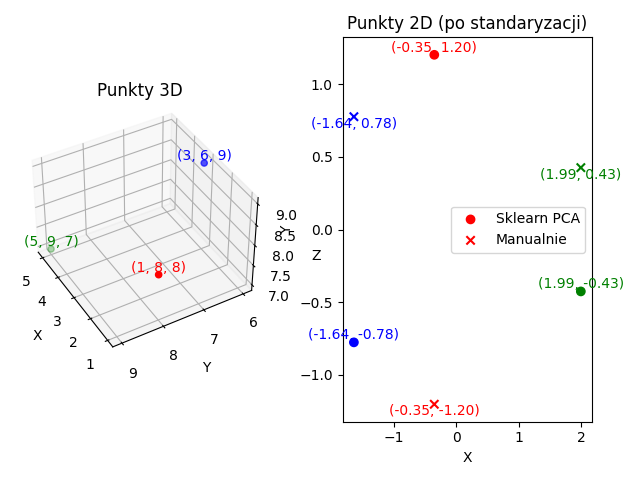
\includegraphics[width=0.8\linewidth]{Zad2/pca.png}
    \caption{Wynik redukcji wymiarów z porównaniem gotowego rozwiązania}
\end{figure}

Wynikowe punkty porównałem z gotową implementacją z biblioteki \textit{sklearn}.
Jak można zauważyć punkty są odbite względem osi y.
Nie zmienia to jednak jakości wyniku,
po prostu drugi wektor własny może być przeciwnie skierowany.

\begin{equation*}
    V_{sklearn} = 
    \begin{bmatrix}
        0.42397 & -0.89385 \\
        0.62384 & 0.40498 \\
        -0.65655 & -0.19240 \\
    \end{bmatrix}
\end{equation*}

\subsection{Wnioski}

Metoda PCA pozwala na redukcję wymiarów danych, nie tracąc przy tym
istotnych informacji o danych. W tym przypadku, po redukcji z 3 do 2 wymiarów,
dane nadal są rozróżnialne, a ich odległości są zachowane. W przypadku
większej liczby wymiarów, metoda PCA pozwala na wybranie tych, które
najbardziej różnicują dane, a pozostałe odrzucić, tak jak w tym 
przypadku odrzucono wektor własny odpowiadający najmniejszej wartości
własnej ($v_3$).

\section{Zadanie 3 - Szukanie minimum funkcji}

Do znalezienia minimum funkcji zdecydowałem się na skorzystanie z
trzech metod iteracyjnych: gradientowej, symulowanego wyżarzania
oraz szukania przypadkowego.

Wybrałem funkcję $f(x, y) = 3(x-1)^2-2(x-1)y+3y^2$. Minimum funkcji to $f(1, 0) = 0$.
Jako punkt startowy dla wszystkich metod wybrałem $X_0 = (-2, 3)$, dokładność
obliczeń ustawiłem na $10^{-4}$ natomiast maksymalną liczbę iteracji równą 5 dla
metody gradientowej, by porównać ją z ręcznie obliczonymi wartościami. Metody
symulowanego wyżarzania i szukania przypadkowego wykonałem dla 1000 iteracji.

\begin{figure}[H]
    \centering
    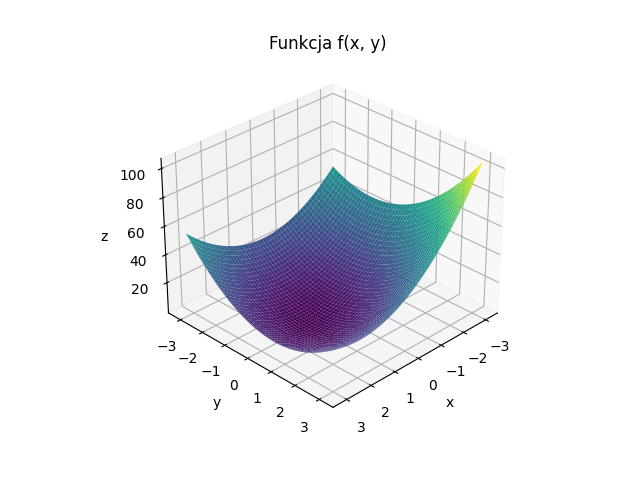
\includegraphics[width=0.7\textwidth]{Zad3/function.png}
    \caption{Wykres funkcji $f(x, y)$}
\end{figure}

\subsection{Metoda gradientowa}

Do wyznaczenia minimum funkcji metodą gradientową trzeba użyć
wzoru:
\begin{equation}
X_{k+1} = X_k - \alpha_k \nabla f(X_k)
\end{equation}
gdzie $\alpha_k$ jest stałą kroku, 
a $\nabla f(X_k)$ jest gradientem
funkcji $f(x, y)$ w punkcie $X_k$.

Gradient funkcji $f(x, y)$ to inaczej wektor pochodnych
cząstkowych:
\begin{equation}
\nabla f(x, y) = \left( \frac{\partial f}{\partial x}, \frac{\partial f}{\partial y} \right)
\end{equation}
W przypadku wybranej funkcji gradient ma postać:
\begin{equation}
\nabla f(x, y) = {6(x - 1)-2y \choose -2(x-1)+6y}
\end{equation}

Dla punktu startowego $X_0 = (-2, 3)$
wyznaczenie 5 kolejnych punktów wygląda następująco:
\begin{equation*}
    \begin{aligned}
    X_1 &= {{-2} \choose {3}} - 0.1 {6(-2 - 1)-2\cdot3 \choose -2\cdot(-2-1)+6\cdot3} = {{0.4} \choose {0.6}} \\
    X_2 &= {{0.4} \choose {0.6}} - 0.1 {6(0.4 - 1)-2\cdot0.6 \choose -2\cdot(0.4-1)+6\cdot0.6} = {{0.88} \choose {0.12}} \\
    X_3 &= {{0.88} \choose {0.12}} - 0.1 {6(0.88 - 1)-2\cdot0.12 \choose -2\cdot(0.88-1)+6\cdot0.12} = {{0.976} \choose {0.024}} \\
    X_4 &= {{0.976} \choose {0.024}} - 0.1 {6(0.976 - 1)-2\cdot0.024 \choose -2\cdot(0.976-1)+6\cdot0.024} = {{0.9952} \choose {0.0048}} \\
    X_5 &= {{0.9952} \choose {0.0048}} - 0.1 {6(0.9952 - 1)-2\cdot0.0048 \choose -2\cdot(0.9952-1)+6\cdot0.0048} = {{0.99904} \choose {0.00096}}
    \end{aligned}
\end{equation*}

Dla tego przykładu wartość funkcji w punkcie $X_5$ wynosi $f(X_5) = 7.3727 \cdot 10^{-6}$.

\subsection{Metoda symulowanego wyżarzania}
Metoda symulowanego wyżarzania polega na losowaniu kolejnych punktów
z pewnego otoczenia punktu $X_k$ i sprawdzaniu czy wartość funkcji
w tym punkcie jest mniejsza niż w poprzednim. Jeśli tak to punkt
$X_{k+1}$ staje się nowym punktem startowym. Jeśli nie to punkt
$X_{k+1}$ jest losowany ponownie. Wraz z kolejnymi iteracjami
otoczenie punktu $X_k$ zmniejsza się. W ten sposób metoda
symulowanego wyżarzania przeszukuje coraz mniejsze obszary
wokół punktu $X_k$.

\subsubsection{Opis kroków}

\begin{enumerate}
    \item Wybranie losowego punktu startowego $X_0$
    \item Wyznaczenie wartości funkcji $f(X_k)$
    \item Wyznaczenie nowego punktu $w'= w + \Delta w$ z otoczenia punktu $X_k$,
    gdzie $\Delta w$ jest realizacją zmiennej losowej o rozkładzie normalnym
    $g(\Delta w,T) = (2 \pi T) ^{-\frac{n}{2}} e^{-\frac{{\Delta w }^2}{2T}}$
    \item Wyznaczenie wartości funkcji $f(w')$
    \item Podstawienie $w'$ za $w$ jeśli $f(w') < f(w)$ lub gdy
    $r < \frac{1}{1 + e^{\frac{\Delta f}{T}}}$, gdzie $r$ jest realizacją zmiennej
    losowej o rozkładzie jednostajnym na przedziale $[0, 1]$
    \item Zmniejszenie temperatury $T' = \alpha T$
    \item Zwiększenie licznika iteracji $k = k + 1$. Zakończenie gdy $k = k_{max}$ lub gdy $f(X_k) < f_{min}$
\end{enumerate}

\subsection{Metoda szukania przypadkowego}
Metoda szukania przypadkowego podobnie jak metoda symulowanego
wyżarzania polega na losowaniu kolejnych punktów z pewnego
otoczenia punktu $X_k$. W tym przypadku zakres losowania
jest stały i nie zmniejsza się wraz z kolejnymi iteracjami.

\subsubsection{Opis kroków}

\begin{enumerate}
    \item Wybranie losowego punktu startowego $X_0$
    \item Wyznaczenie wartości funkcji $f(X_k)$
    \item Wyznaczenie nowego punktu $w'= w + \Delta w$ z otoczenia punktu $X_k$,
    gdzie $\Delta w$ jest realizacją zmiennej losowej o rozkładzie normalnym
    $g(\Delta w,\sigma) = (2 \pi \sigma) ^{-\frac{n}{2}} e^{-\frac{{\Delta w }^2}{2\sigma}}$
    (w tym przypadku $\sigma = const$)
    \item Wyznaczenie wartości funkcji $f(w')$
    \item Podstawienie $w'$ za $w$ jeśli $f(w') < f(w)$ 
    \item Zwiększenie licznika iteracji $k = k + 1$. Zakończenie gdy $k = k_{max}$ lub gdy $f(X_k) < f_{min}$
\end{enumerate}

\subsection{Wykresy}

\begin{figure}[H]
    \centering
    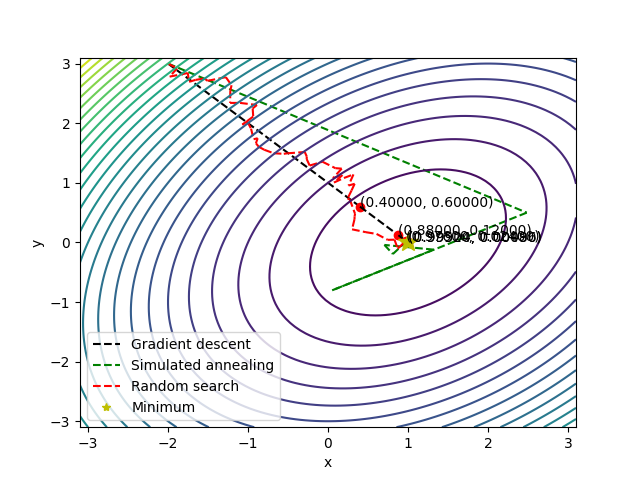
\includegraphics[width=0.7\textwidth]{Zad3/plot.png}
    \caption{Rzut 2D wykresu funkcji $f(x, y)$ wraz z 
    wyznaczonymi minimami od iteracji dla trzech metod}
\end{figure}

\begin{figure}[H]
    \centering
    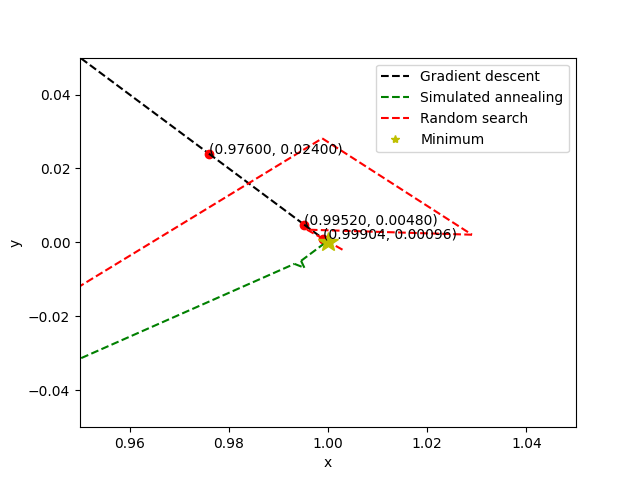
\includegraphics[width=0.7\textwidth]{Zad3/plot_zoomed.png}
    \caption{Zbliżenie wykresu funkcji $f(x, y)$ wokół minimum}
\end{figure}

\subsection{Wnioski}
W porównaniu metod gradientowych, wyżarzania oraz szukania 
przypadkowego można wyróżnić kilka wniosków:

Metoda gradientowa jest najskuteczniejsza, gdyż pozwala na znalezienie 
globalnego minimum, jeśli funkcja jest różniczkowalna i nie ma zbyt 
wiele minimów lokalnych. Metoda ta działa dobrze dla prostych funkcji, 
ale może mieć problemy z funkcjami nieliniowymi, 
gdzie minimum globalne znajduje się w dolinie.

Metoda wyżarzania jest skuteczna, ale wymaga więcej czasu niż metoda 
gradientowa. Ważnym czynnikiem jest dobór temperatury początkowej,
jak również stopnia jej zmniejszania.
W przeciwieństwie do metody gradientowej, metoda 
wyżarzania nie zawsze znajduje globalne minimum, ale może znaleźć 
rozwiązanie optymalne dla funkcji, które mają wiele minimów lokalnych. 

Metoda szukania przypadkowego jest najmniej skuteczna, ale jest najprostsza do 
zastosowania. Ta metoda działa dobrze dla funkcji, które mają wiele 
minimów lokalnych, ale może trwać bardzo długo, zanim znajdzie się 
globalne minimum. W rzeczywistości, jeśli funkcja ma więcej niż 
kilka wymiarów, szansa na znalezienie globalnego minimum jest bardzo niska.
W związku z powyższymi wnioskami, wybór odpowiedniej metody optymalizacji 
zależy od charakterystyki funkcji, której minimum poszukujemy, 
a także od czasu, jaki mamy na wykonanie obliczeń. 

\section{Zadanie 4 - Sieć neuronowa}

Zadaniem jest zbudowanie sieci neuronowej, która będzie rozwiązywać
pewien zdefiniowany problem. Zdecydowałem się na rozwiązanie problemu klasyfikacji
punktów w przestrzeni 2D. Model ma rozpoznawać czy dany punkt należy
do zdefiniowanej wcześniej figury czy nie.

Wybrałem trapez opisany za pomocą tych czterech równań:
\begin{equation}
    \begin{cases}
        -\frac{2}{3}x_1 - x_2 + 4 = 0 \\
        \frac{1}{2}x_1 - x_2 = 0 \\
        \frac{1}{2}x_1 - x_2 + 3 = 0 \\
        -\frac{3}{2}x_1 - x_2 + 14 = 0
    \end{cases}
\end{equation}
\begin{figure}[H]
    \centering
    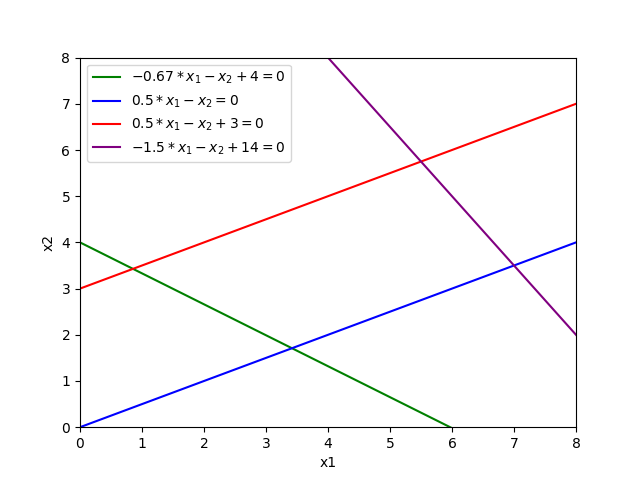
\includegraphics[width=0.6\textwidth]{Zad4/trapez.png}
    \caption{Wykres trapezu wykorzystywanego do tego zadania}
\end{figure}

\subsection{Opis budowy sieci neuronowej}

Sieć składa się z 2 warstw. Pierwsza warstwa ma 4 neurony odpowiadające
czterem równaniom, które opisują trapez. Druga warstwa ma jeden neuron, który
ma za zadanie zwrócić 1 jeśli punkt jest wewnątrz trapezu lub 0 jeśli punkt
jest na zewnątrz.

Pojedynczy neuron warstwy pierwszej można opisać równaniem:
\begin{equation}
    \sigma(w_1x_1 + w_2x_2 + w_3)
\end{equation}
gdzie $w_i$ to wagi, $x_i$ to wejścia, a $\sigma$ to funkcja
aktywacji. 

W tym przypadku jako funkcję aktywacji użyłem funkcji stepu (hardlim):
\begin{equation}
    \sigma(x) = \begin{cases}
        1 & \text{dla } x > 0 \\
        0 & \text{dla } x \leq 0
    \end{cases}
\end{equation}

Wagi neuronów są następujące:

\begin{table}[H]
    \centering
    \begin{tabular}{c c c}
        $w_{11} = \cfrac{2}{3}$ & $w_{12} = 1$ & $w_{13} = -4$ \\
        $w_{21} = -\cfrac{1}{2}$ & $w_{22} = 1$ & $w_{23} = 0$ \\
        $w_{31} = \cfrac{1}{2}$ & $w_{32} = -1$ & $w_{33} = 3$ \\
        $w_{41} = -\cfrac{3}{2}$ & $w_{42} = -1$ & $w_{43} = 14$ \\
    \end{tabular}
\end{table}

Wagi neuronów 1. i 2. zostały przemnożone przez -1, ponieważ
w tym przypadku chcemy, żeby punkt znajdował się nad prostą,
a nie pod nią.

Piąty neuron jest opisany równaniem:
\begin{equation}
    \sigma(w_1N_1 + w_2N_2 + w_3N_3 + w_4N_4 + w_5\cdot1)
\end{equation}
gdzie $N_i$ to wyjścia z neuronów pierwszej warstwy, a $w_i$ to wagi.

Wagi piątego neuronu zostały dobrane w taki sposób, by każdy neuron pierwszej warstwy zwracał
1, gdy punkt znajduje się po poprawnej stronie prostej, którą opisują. 
Wyglądają następująco:
\begin{equation}
    w_{51} = w_{52} = w_{53} = w_{54} = 1 \quad w_{55} = -3
\end{equation}

Waga biasa została ustawiona jako -3, ponieważ gdy wszystkie neurony
pierwszej warstwy zwrócą 1 (punkt znajduje się wewnątrz trapezu), to piąty
neuron również zwróci 1. W każdym innym przypadku zwróci 0.

\begin{figure}[H]
    \centering
    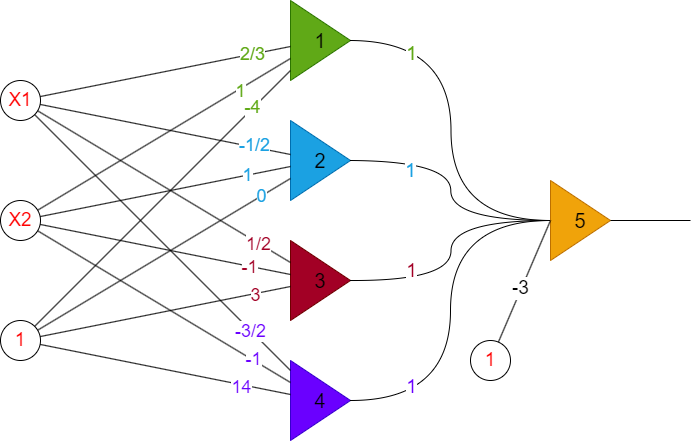
\includegraphics[width=0.9\textwidth]{Zad4/sieć.png}
    \caption{Schemat sieci neuronowej}
\end{figure}

\subsection{Zasada działania modelu}

Zasadę działania modelu można opisać następująco dla przykładowcych punktów:

\begin{itemize}
    \centering
    \item $P_1 = (4, 3)$
    \item $P_2 = (7, 2)$
\end{itemize}
Dla punktu $P_1$ neurony zwracają następujące wartości:
\begin{itemize}
    \centering
    \item $N_1 = \sigma(\frac{2}{3}\cdot4 + 3 - 4) = \sigma(\frac{5}{3}) = 1$
    \item $N_2 = \sigma(-\frac{1}{2}\cdot4 + 3) = \sigma(1) = 1$
    \item $N_3 = \sigma(\frac{1}{2}\cdot4 - 3 + 3) = \sigma(2) = 1$
    \item $N_4 = \sigma(-\frac{3}{2}\cdot4 - 3 + 14) = \sigma(5) = 1$
    \item $N_5 = \sigma(1 + 1 + 1 + 1 - 3) = \sigma(1) = 1$
\end{itemize}
Według tej sieci punkt $P_1$ znajduje się wewnątrz trapezu.

Natomiast dla punktu $P_2$:
\begin{itemize}
    \centering
    \item $N_1 = \sigma(\frac{2}{3}\cdot7 + 2 - 4) = \sigma(\frac{8}{3}) = 1$
    \item $N_2 = \sigma(-\frac{1}{2}\cdot7 + 2) = \sigma(-\frac{3}{2}) = 0$
    \item $N_3 = \sigma(\frac{1}{2}\cdot7 - 2 + 3) = \sigma(\frac{9}{2}) = 1$
    \item $N_4 = \sigma(-\frac{3}{2}\cdot7 - 2 + 14) = \sigma(\frac{3}{2}) = 1$
    \item $N_5 = \sigma(1 + 0 + 1 + 1 - 3) = \sigma(0) = 0$
\end{itemize}
Według tej sieci punkt $P_2$ znajduje się na zewnątrz trapezu.

\subsection{Test modelu teoretycznego}

Do przetestowania modelu teoretycznego, wykorzystałem bibliotekę
\textit{keras}. Wylosowałem 1000 punktów z przedziału $[0, 8]$ i
przetestowałem je na sieci, której wagi są wyznaczone przez
równania prostych. Wyniki przedstawia poniższy wykres:

\begin{figure}[H]
    \centering
    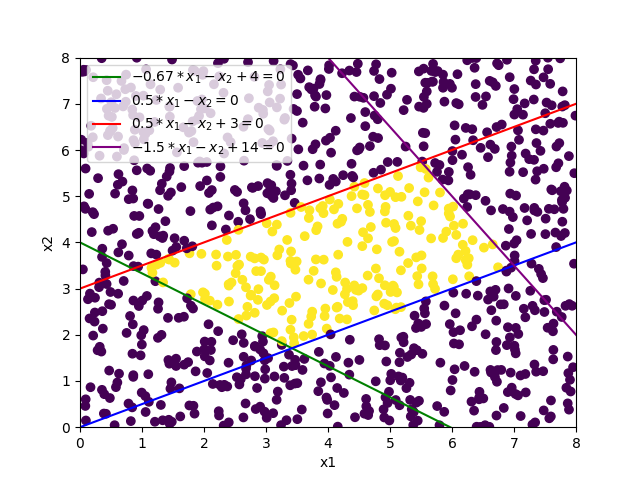
\includegraphics[width=0.6\textwidth]{Zad4/punkty_teor.png}
    \caption{Wykres punktów z zaznaczoną predykcją dla modelu teoretycznego}
\end{figure}

\subsection{Porównanie modelu teoretycznego z gotowym modelem}

Do porównania modelu teoretycznego z gotowym modelem wykorzystałem
ponownie bibliotekę \textit{keras}. Ponownie również wylosowałem
1000 punktów z przedziału $[0, 8]$, które służyły do trenowania modelu.

Jako funkcję aktywacji wybrałem funkcję \textit{hard\_sigmoid}, natomiast
jako funkcję straty wybrałem \textit{mse}. Struktura sieci jest identyczna
jak w modelu teoretycznym. Ilość epok trenowania ustawiłem na 200.

\begin{figure}[H]
    \centering
    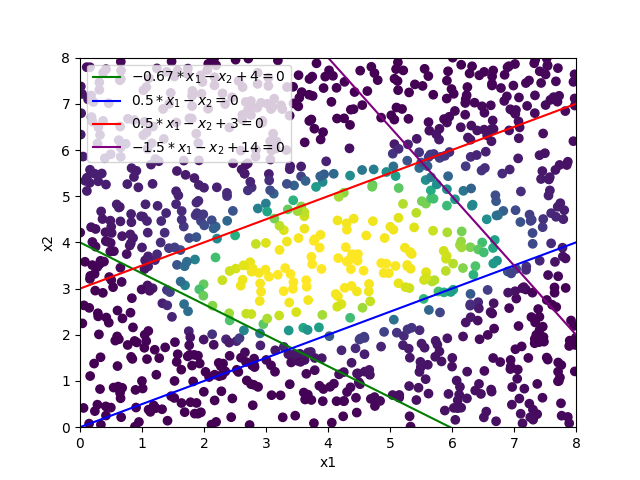
\includegraphics[width=0.6\textwidth]{Zad4/punkty.png}
    \caption{Wykres punktów testowych z zaznaczoną predykcją dla gotowego modelu}
\end{figure}


Dla warstwy pierwszej:

Model zdecydował o wybraniu następujących wag:
\begin{equation*}
    \begin{bmatrix}
        w_{11} & w_{21} & w_{31} & w_{41} \\
        w_{12} & w_{22} & w_{32} & w_{42} \\
    \end{bmatrix}
    =
    \begin{bmatrix}
        0.61588454 & -1.7075858 & 1.7044008 & 0.84863913 \\
        -2.6946127 & 1.419755 & 2.1215165 & 0.84165674 \\
    \end{bmatrix}
\end{equation*}

Oraz następujących wag biasa:
\begin{equation*}
    \begin{bmatrix}
        w_{13} & w_{23} & w_{33} & w_{43}
    \end{bmatrix}
    =
    \begin{bmatrix}
        4.0605855 & -0.993487 & -8.304987 & -8.799887
    \end{bmatrix}
\end{equation*}

Natomiast dla drugiej warstwy:

Model zdecydował o wybraniu następujących wag:
\begin{equation*}
    \begin{bmatrix}
        w_{51} \\
        w_{52} \\
        w_{53} \\
        w_{54} \\
    \end{bmatrix}
    =
    \begin{bmatrix}
        -9.39592 \\
        -9.043343 \\
        4.606038 \\
        -10.647419 \\
    \end{bmatrix}
\end{equation*}

Oraz następującej wagi biasa:
\begin{equation*}
    \begin{bmatrix}
        w_{55}
    \end{bmatrix}
    =
    \begin{bmatrix}
        2.3153777
    \end{bmatrix}
\end{equation*}

Dokładność modelu wyniosła $96.3 \% $.

\subsection{Wnioski}

Jak widać na wykresach, oba modele dobrze radzą sobie z klasyfikacją,
jednakże model teoretyczny jest bardziej dokładny. Wynika to z faktu,
że model teoretyczny korzysta już ze znanych równań prostych, natomiast
model gotowy musi nauczyć się tych równań samodzielnie. 

Ważnym czynnikiem w przypadku modelu gotowego jest również wybór odpowiedniej
funkcji aktywacji oraz funkcji straty, jak również ilości epok, które 
znacząco wpływają na dokładność modelu.

\section{Zadanie 5 - Klasyfikator Bayesa}

\subsection{Opis klasyfikatora}

Klasyfikator Bayesa oparty jest na twierdzeniu Bayesa, 
które jest podstawą teorii prawdopodobieństwa. Zakłada 
się, że obserwacje są niezależne i pochodzą z pewnego 
rozkładu prawdopodobieństwa. Klasyfikator Bayesa 
wykorzystuje te informacje, aby obliczyć prawdopodobieństwo 
przynależności danej obserwacji do poszczególnych klas.

Załóżmy, że mamy zbiór danych uczących składający się z 
obserwacji $d$ i odpowiadających im etykiet klas $C$. 
Klasyfikator Bayesa szacuje prawdopodobieństwo warunkowe 
$P(C_i|d)$, czyli prawdopodobieństwo przynależności i-tej
klasy do obserwacji. 
Twierdzenie Bayesa, które wykorzystuje klasyfikator,
można wyrazić wzorem:

\begin{equation}
    P(C_i|d) = \frac{P(C_i)P(d|C_i)}{P(d)}
\end{equation}
Po zamianie obserwacji $d$ na wektor cech $w$ otrzymujemy:

\begin{equation}
    P(C_i|w_1, w_2, ..., w_n) = \frac{P(C_i)P(w_1, w_2, ..., w_n|C_i)}{P(w_1, w_2, ..., w_n)}
\end{equation}
co można przedstawić w postaci:

\begin{equation}
    P(C_i|w_1, w_2, ..., w_n) = \frac{P(C_i)\prod_{j=1}^{n}P(w_j|C_i)}{P(w_1, w_2, ..., w_n)}
\end{equation}
gdzie:
\begin{itemize}
    \item $P(C_i)$ - prawdopodobieństwo wystąpienia i-tej klasy, wyrażona jako 
    stosunek liczby obserwacji ze znaną i-tą klasą do liczby wszystkich obserwacji
    należących do $m$ klas:
    $P(C_i) = \cfrac{|C_i|}{\sum_{j=1}^{m}|C_j|}$
    \item $P(w_j|C_i)$ - prawdopodobieństwo wystąpienia j-tej cechy w i-tej klasie,
    wyrażona jako stosunek liczby obserwacji z i-tą klasą, w których występuje j-ta cecha,
    do liczby wszystkich obserwacji z i-tą klasą:
    $P(w_j|C_i) = \cfrac{|w_j, C_i|}{|C|}$
\end{itemize}

By uniknąć problemu z zerowymi prawdopodobieństwami,
które mogą wystąpić, gdy na przykład w zbiorze uczącym nie ma obserwacji
z daną cechą, stosuje się wygładzanie Laplace'a. Polega ono
na wyznaczeniu stosunku liczby wystąpień danej cechy w danej klasie
powiększonej o 1, do liczby wszystkich niezerowych cech w danej klasie powiększonej
o liczbę wszystkich cech w zbiorze uczącym.

\begin{equation}\label{eq:eq1}
    P(w_j|C_i) = \cfrac{|w_j, C_i| + 1}{|w, C_i| + |v|}
\end{equation}

Po wyznaczeniu prawdopodobieństw warunkowych $P(C_i|w_1, w_2, ..., w_n)$ dla każdej klasy
$C_i$ klasyfikator Bayesa przypisuje obserwację $d$ do klasy $C_i$, dla której prawdopodobieństwo
warunkowe jest największe (z zasady maksimum a posteriori).

\begin{equation}
    C_{pred} = \arg\max_{i}P(C_i|w_1, w_2, ..., w_n)
\end{equation}

\subsection{Zadanie}

Przygotowałem przykładowe dane do obliczeń. Zadaniem jest
sklasyfikowanie obserwacji $d_7$ do jednej z 4 klas $C_1$, $C_2$, $C_3$ oraz $C_4$.

\begin{table}[H]
    \centering
    \begin{tabular}{|c|c|c|c|c|c|c|}
        \hline
        Obserwacja & $w_1$ & $w_2$ & $w_3$ & $w_4$ & $w_5$ & Klasa \\
        \hline
        $d_1$ & 0 & 1 & 1 & 0 & 0 & $C_1$ \\
        \hline
        $d_2$ & 1 & 1 & 0 & 0 & 1 & $C_2$ \\
        \hline
        $d_3$ & 1 & 0 & 0 & 0 & 1 & $C_2$ \\
        \hline
        $d_4$ & 0 & 0 & 1 & 1 & 1 & $C_3$ \\
        \hline
        $d_5$ & 1 & 1 & 1 & 1 & 1 & $C_3$ \\
        \hline
        $d_6$ & 0 & 1 & 0 & 1 & 0 & $C_4$ \\
        \hline
        $d_7$ & 1 & 0 & 1 & 0 & 0 & ? \\
        \hline
    \end{tabular}
\end{table}

Na początku należy wyznaczyć prawdopodobieństwa wystąpienia każdej z klas $C_i$.

\begin{equation}
    P(C_1) = \cfrac{1}{6} \quad P(C_2) = \cfrac{1}{3} \quad P(C_3) = \cfrac{1}{3} \quad P(C_4) = \cfrac{1}{6}
\end{equation}

Następnie korzystając z równania \ref{eq:eq1}. wyznaczamy prawdopodobieństwa
wystąpienia każdej z cech $w_j$ w każdej z klas $C_i$.

\subsubsection*{Klasa $C_1$}

\begin{equation*}
    P(w_1|C_1) = \frac{0 + 1}{2 + 5} = \frac{1}{7} \quad P(w_2|C_1) = \frac{1 + 1}{2 + 5} = \frac{2}{7}
\end{equation*}

\begin{equation*}
    P(w_3|C_1) = \frac{1 + 1}{2 + 5} = \frac{2}{7} \quad P(w_4|C_1) = \frac{0 + 1}{2 + 5} = \frac{1}{7} \quad P(w_5|C_1) = \frac{0 + 1}{2 + 5} = \frac{1}{7}
\end{equation*}

\subsubsection*{Klasa $C_2$}

\begin{equation*}
    P(w_1|C_2) = \frac{2 + 1}{5 + 5} = \frac{3}{10} \quad P(w_2|C_2) = \frac{1 + 1}{5 + 5} = \frac{2}{10} = \frac{1}{5}
\end{equation*}

\begin{equation*}
    P(w_3|C_2) = \frac{0 + 1}{5 + 5} = \frac{1}{10} \quad P(w_4|C_2) = \frac{0 + 1}{5 + 5} = \frac{1}{10} \quad P(w_5|C_2) = \frac{2 + 1}{5 + 5} = \frac{3}{10}
\end{equation*}

\subsubsection*{Klasa $C_3$}

\begin{equation*}
    P(w_1|C_3) = \frac{1 + 1}{8 + 5} = \frac{2}{13} \quad P(w_2|C_3) = \frac{2 + 1}{8 + 5} = \frac{3}{13}
\end{equation*}

\begin{equation*}
    P(w_3|C_3) = \frac{2 + 1}{8 + 5} = \frac{3}{13} \quad P(w_4|C_3) = \frac{2 + 1}{8 + 5} = \frac{3}{13} \quad P(w_5|C_3) = \frac{2 + 1}{8 + 5} = \frac{3}{13}
\end{equation*}
    
\subsubsection*{Klasa $C_4$}

\begin{equation*}
    P(w_1|C_4) = \frac{0 + 1}{2 + 5} = \frac{1}{7} \quad P(w_2|C_4) = \frac{1 + 1}{2 + 5} = \frac{2}{7}
\end{equation*}

\begin{equation*}
    P(w_3|C_4) = \frac{0 + 1}{2 + 5} = \frac{1}{7} \quad P(w_4|C_4) = \frac{1 + 1}{2 + 5} = \frac{2}{7} \quad P(w_5|C_4) = \frac{0 + 1}{2 + 5} = \frac{1}{7}
\end{equation*}

Ostatnim krokiem jest wyznaczenie prawdopodobieństwa przynależności obserwacji $d_7$
do każdej z klas $C_i$ i wybranie klasy o największym prawdopodobieństwie.
Interesują nas tylko niezerowe cechy obserwacji $d_7$, czyli $w_1$ i $w_3$.

\begin{equation}
    P(C_i|d_7) = P(C_i) \cdot P(w_1|C_i) \cdot P(w_3|C_i)
    \label{eq:eq2}
\end{equation}

\begin{equation*}
    P(C_1|d_7) = P(C_1) \cdot P(w_1|C_1) \cdot P(w_3|C_1) = \frac{1}{6} \cdot \frac{1}{7} \cdot \frac{2}{7} = \frac{2}{294}
\end{equation*}

\begin{equation*}
    P(C_2|d_7) = P(C_2) \cdot P(w_1|C_2) \cdot P(w_3|C_2) = \frac{1}{3} \cdot \frac{3}{10} \cdot \frac{1}{10} = \frac{3}{300}
\end{equation*}

\begin{equation*}
    P(C_3|d_7) = P(C_3) \cdot P(w_1|C_3) \cdot P(w_3|C_3) = \frac{1}{3} \cdot \frac{2}{13} \cdot \frac{3}{13} = \frac{6}{507}
\end{equation*}

\begin{equation*}
    P(C_4|d_7) = P(C_4) \cdot P(w_1|C_4) \cdot P(w_3|C_4) = \frac{1}{6} \cdot \frac{1}{7} \cdot \frac{1}{7} = \frac{1}{294}
\end{equation*}

\begin{equation*}
    P(C_1|d_7) = \frac{2}{294} \approx 0.0068 \quad P(C_2|d_7) = \frac{3}{300} = 0.01
\end{equation*}

\begin{equation*}
    P(C_3|d_7) = \frac{6}{507} \approx 0.0118 \quad P(C_4|d_7) = \frac{1}{294} \approx 0.0034
\end{equation*}

\begin{equation*}
    P(C_3|d_7) > P(C_2|d_7) > P(C_1|d_7) > P(C_4|d_7)
\end{equation*}

\begin{equation*}
    d_7 \in C_3
\end{equation*}

Obserwacja $d_7$ została zaklasyfikowana do klasy $C_3$.

\subsection{Wnioski}

Klasyfikator Bayesa może być niewystarczający w przypadku, gdy w zbiorze uczącym
nie ma wystarczającej liczby obserwacji, które zawierają wszystkie cechy. W tym przypadku
klasyfikator jest tylko w $1.18\%$ pewny, że obserwacja $d_7$ należy do klasy $C_3$,
co dla niektórych zastosowań może być niewystarczające. Natomiast implementacja
klasyfikatora jest bardzo prosta i nie wymaga wielu obliczeń, co jest jego dużą zaletą.



\end{document}